% GNUPLOT: LaTeX picture with Postscript
\begingroup
  \makeatletter
  \providecommand\color[2][]{%
    \GenericError{(gnuplot) \space\space\space\@spaces}{%
      Package color not loaded in conjunction with
      terminal option `colourtext'%
    }{See the gnuplot documentation for explanation.%
    }{Either use 'blacktext' in gnuplot or load the package
      color.sty in LaTeX.}%
    \renewcommand\color[2][]{}%
  }%
  \providecommand\includegraphics[2][]{%
    \GenericError{(gnuplot) \space\space\space\@spaces}{%
      Package graphicx or graphics not loaded%
    }{See the gnuplot documentation for explanation.%
    }{The gnuplot epslatex terminal needs graphicx.sty or graphics.sty.}%
    \renewcommand\includegraphics[2][]{}%
  }%
  \providecommand\rotatebox[2]{#2}%
  \@ifundefined{ifGPcolor}{%
    \newif\ifGPcolor
    \GPcolortrue
  }{}%
  \@ifundefined{ifGPblacktext}{%
    \newif\ifGPblacktext
    \GPblacktexttrue
  }{}%
  % define a \g@addto@macro without @ in the name:
  \let\gplgaddtomacro\g@addto@macro
  % define empty templates for all commands taking text:
  \gdef\gplbacktext{}%
  \gdef\gplfronttext{}%
  \makeatother
  \ifGPblacktext
    % no textcolor at all
    \def\colorrgb#1{}%
    \def\colorgray#1{}%
  \else
    % gray or color?
    \ifGPcolor
      \def\colorrgb#1{\color[rgb]{#1}}%
      \def\colorgray#1{\color[gray]{#1}}%
      \expandafter\def\csname LTw\endcsname{\color{white}}%
      \expandafter\def\csname LTb\endcsname{\color{black}}%
      \expandafter\def\csname LTa\endcsname{\color{black}}%
      \expandafter\def\csname LT0\endcsname{\color[rgb]{1,0,0}}%
      \expandafter\def\csname LT1\endcsname{\color[rgb]{0,1,0}}%
      \expandafter\def\csname LT2\endcsname{\color[rgb]{0,0,1}}%
      \expandafter\def\csname LT3\endcsname{\color[rgb]{1,0,1}}%
      \expandafter\def\csname LT4\endcsname{\color[rgb]{0,1,1}}%
      \expandafter\def\csname LT5\endcsname{\color[rgb]{1,1,0}}%
      \expandafter\def\csname LT6\endcsname{\color[rgb]{0,0,0}}%
      \expandafter\def\csname LT7\endcsname{\color[rgb]{1,0.3,0}}%
      \expandafter\def\csname LT8\endcsname{\color[rgb]{0.5,0.5,0.5}}%
    \else
      % gray
      \def\colorrgb#1{\color{black}}%
      \def\colorgray#1{\color[gray]{#1}}%
      \expandafter\def\csname LTw\endcsname{\color{white}}%
      \expandafter\def\csname LTb\endcsname{\color{black}}%
      \expandafter\def\csname LTa\endcsname{\color{black}}%
      \expandafter\def\csname LT0\endcsname{\color{black}}%
      \expandafter\def\csname LT1\endcsname{\color{black}}%
      \expandafter\def\csname LT2\endcsname{\color{black}}%
      \expandafter\def\csname LT3\endcsname{\color{black}}%
      \expandafter\def\csname LT4\endcsname{\color{black}}%
      \expandafter\def\csname LT5\endcsname{\color{black}}%
      \expandafter\def\csname LT6\endcsname{\color{black}}%
      \expandafter\def\csname LT7\endcsname{\color{black}}%
      \expandafter\def\csname LT8\endcsname{\color{black}}%
    \fi
  \fi
  \setlength{\unitlength}{0.0500bp}%
  \begin{picture}(7200.00,5040.00)%
    \gplgaddtomacro\gplbacktext{%
      \csname LTb\endcsname%
      \put(540,830){\makebox(0,0)[r]{\strut{}0}}%
      \put(540,1780){\makebox(0,0)[r]{\strut{}0.5}}%
      \put(540,2729){\makebox(0,0)[r]{\strut{}1}}%
      \put(1023,440){\makebox(0,0){\strut{} 0}}%
      \put(1932,440){\makebox(0,0){\strut{} 0.5}}%
      \put(2841,440){\makebox(0,0){\strut{} 1}}%
      \put(3749,440){\makebox(0,0){\strut{} 1.5}}%
      \put(4658,440){\makebox(0,0){\strut{} 2}}%
      \put(5567,440){\makebox(0,0){\strut{} 2.5}}%
      \put(6476,440){\makebox(0,0){\strut{} 3}}%
      \put(1023,4639){\makebox(0,0){\strut{}0}}%
      \put(2841,4639){\makebox(0,0){\strut{}300}}%
      \put(4658,4639){\makebox(0,0){\strut{}600}}%
      \put(6476,4639){\makebox(0,0){\strut{}900}}%
      \put(200,1739){\rotatebox{-270}{\makebox(0,0){\strut{}Transmission}}}%
      \put(3749,140){\makebox(0,0){\strut{}Phase $\nicefrac{\phi}{\pi}$}}%
      \put(3749,4938){\makebox(0,0){\strut{}Frequenz $\nu$ [MHz]}}%
      \put(1750,2957){\makebox(0,0)[l]{\strut{}FSR}}%
    }%
    \gplgaddtomacro\gplfronttext{%
      \csname LTb\endcsname%
      \put(1620,4226){\makebox(0,0)[r]{\strut{}$F=2$}}%
      \csname LTb\endcsname%
      \put(1620,3926){\makebox(0,0)[r]{\strut{}$F=10$}}%
      \csname LTb\endcsname%
      \put(1620,3626){\makebox(0,0)[r]{\strut{}$F=100$}}%
    }%
    \gplgaddtomacro\gplbacktext{%
      \csname LTb\endcsname%
      \put(3756,3368){\makebox(0,0)[r]{\strut{} 0}}%
      \put(3756,3677){\makebox(0,0)[r]{\strut{} 50}}%
      \put(3756,3986){\makebox(0,0)[r]{\strut{} 100}}%
      \put(3756,4295){\makebox(0,0)[r]{\strut{} 150}}%
      \put(3876,2921){\makebox(0,0){\strut{} 0}}%
      \put(4440,2921){\makebox(0,0){\strut{} 0.2}}%
      \put(5004,2921){\makebox(0,0){\strut{} 0.4}}%
      \put(5567,2921){\makebox(0,0){\strut{} 0.6}}%
      \put(6131,2921){\makebox(0,0){\strut{} 0.8}}%
      \put(6695,2921){\makebox(0,0){\strut{} 1}}%
      \put(3356,3708){\rotatebox{-270}{\makebox(0,0){\strut{}Finesse}}}%
      \put(5285,3280){\makebox(0,0){\strut{}Reflektivit{"a}t}}%
    }%
    \gplgaddtomacro\gplfronttext{%
    }%
    \gplbacktext
    \put(0,0){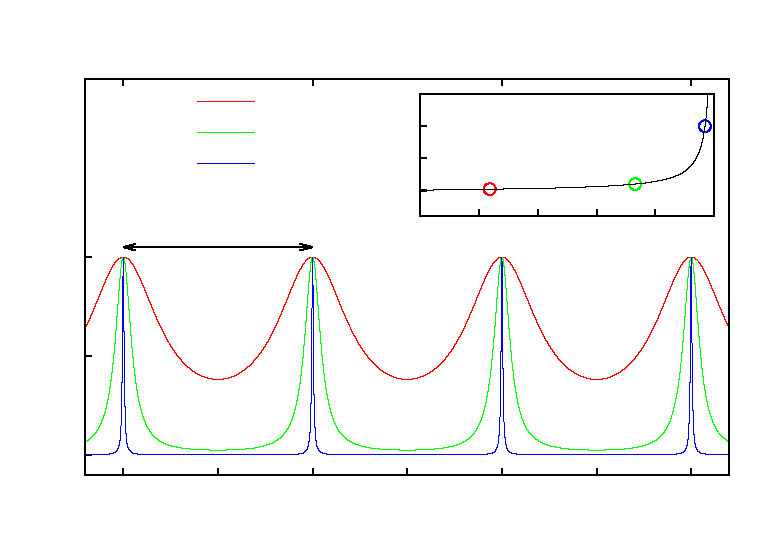
\includegraphics{airy-funktion}}%
    \gplfronttext
  \end{picture}%
\endgroup
